\documentclass[a4paper,10pt,xcolor=pdftex,dvipsnames,table]{beamer}
\mode<presentation> {
		\usetheme{Madrid}
		\usecolortheme[]{beaver}
%		\usecolortheme[]{seahorse}
%		\usecolortheme[]{dolphin}
		\usefonttheme{professionalfonts}
%		\usefonttheme[onlysmall]{structurebold}				% use smallcaps in bold structures (not everywhere)
%		\usefonttheme[frametitle]{structuresmallcapsserif}
%		\usetheme[headline=sections,frametitle=normal,titlepage=picture]{progressbar}
%		\useinnertheme{progressbar}
%		\useoutertheme{progressbar}
        \useoutertheme{progressbar}
        \setbeamertemplate{blocks}[rounded][shadow=false]
        \useinnertheme{rounded}    % circles, inmargin, rectangles, rounded
%        \newcommand{\includeoptional}{false}
        \newcommand{\includeoptional}{true}
		\setbeamertemplate{headline}{}
        \setbeamertemplate{navigation symbols}{}
%		\setbeamertemplate{frametitle}{}
%		\setbeamertemplate{footline}{}
		\setbeamersize{text margin right=1cm} % erzeugt einen Randabstand
        \setbeamercovered{transparent}
}

\mode<handout>{
  \usetheme{Pittsburgh}
  \usecolortheme[]{default}
%  \usecolortheme{albatross}
%  \usecolortheme{beaver}
%  \usecolortheme{beetle}
%  \usecolortheme{crane}
%  \usecolortheme{dolphin}
%  \usecolortheme{dove}
%  \usecolortheme{fly}
%  \usecolortheme{lily}
%  \usecolortheme{orchid}
%  \usecolortheme{rose}
%  \usecolortheme{seagull}
%  \usecolortheme{seahorse}
%  \usecolortheme{whale}
%  \usecolortheme{wolverine}
    \useinnertheme{progressbar}
    		\setbeamertemplate{headline}{}
		\setbeamertemplate{footline}{}
}

\usepackage{pgfpages}
\usepackage{color, german, graphicx}
\usepackage{eurosym}
\usepackage{fancyvrb} % use \begin{frame}[fragile] !
\usepackage{xmpmulti}
\usepackage{setspace}
\selectlanguage{english}
\usepackage{pslatex}
\usepackage{ulem}
\usepackage[absolute,overlay]{textpos}
\usepackage{graphicx}
\usepackage{ifthen} 
\usepackage{hyperref}
\usepackage{tabu}
\hypersetup{%
    colorlinks=true, linktocpage=true, pdfstartpage=1, pdfstartview=FitV,pdfpagelayout=TwoPageRight,%
    breaklinks=true, pdfpagemode=UseNone, pageanchor=true, pdfpagemode=UseOutlines,%
    plainpages=false, bookmarksnumbered, bookmarksopen=true, bookmarksopenlevel=2,%
    hypertexnames=true, pdfhighlight=/O, urlcolor=footersymbolcolor, %
    pdftitle={Tools \& Databases of Short Linear Motifs}
    pdfauthor={Holger Dinkel},%
    pdfsubject={Tools \& Databases of Short Linear Motifs}
    pdfkeywords={Short Linear Motif},%
    pdfcreator={pdfLaTeX},%
    pdfproducer={LaTeX}%
}

\newcommand\Paper[3]{%
%\begin{textblock*}{.98\textwidth}(5pt,.98\textheight)%
\begin{textblock*}{.98\textwidth}(5pt,\textheight)%
 \begin{spacing}{.5} 
{\sc\scriptsize \textsl{''\raggedright #1``};
{\tiny #2; (#3)}}
\end{spacing}
\end{textblock*}}
%\setbeameroption{show notes on second screen=right}

%\listfiles 

\begin{document}
%\date{}
\date{EMBO Practical Course Computational analysis of protein-protein interactions: From sequences to networks}


\title{Tools \& Databases of Short Linear Motifs}
\subtitle{}
\author{Holger Dinkel}

%\setbeamercolor{background canvas}{bg=} %=ohne Hintergrund

\definecolor{paleblue}{RGB}{100,100,170} 
%\setbeamercolor{description item}{fg=emblrot}
%
\setbeamerfont{block title alerted}{size=\small}
\setbeamerfont{block body alerted}{size=\footnotesize}
\setbeamerfont{block title}{size=\small}
\setbeamerfont{block body}{size=\footnotesize}
%
\setbeamerfont{structure}{series=\bfseries} % make structure text bold
\setbeamerfont{alerted text}{series=\bfseries} % make alerted text bold
\setbeamerfont{note page}{size=\scriptsize} % make the note text smaller
\setbeamerfont{note text}{size=\scriptsize}
\setbeamerfont{footnote}{size=\tiny}
\setbeamerfont{caption}{size=\scriptsize}
\setbeamerfont{description}{series=\bfseries} % make alerted text bold
\setbeamerfont{description item}{series=\bfseries} % make alerted text bold
\setbeamerfont{frametitle}{size=\normalfont,shape=\scshape}

\newcommand{\optional}[1]{\ifthenelse{\equal{\includeoptional}{true}}{#1}{---}}
\pgfdeclareimage[height=6.5mm]{elmlogo}{elm_logo_transparent.png}
\pgfdeclareimage[height=6.5mm]{embllogo}{EMBL-Logo-only_border.png}
\pgfdeclareimage[height=6.5mm]{phosphoelmlogo}{images/Phospho/Phospho_ELM_logo.png}
\pgfdeclareimage[height=6.5mm]{phosphositepluslogo}{images/Phospho/phosphositeplus_logo.png}
\pgfdeclareimage[height=5mm]{switcheslogo}{images/switches/switches_elm_logo.png}

\newcommand{\PROT}[1]{\textsc{#1}}
\newcommand{\hogsboxtop}[2]{
\begin{minipage}[t]{.99\textwidth}   
\begin{exampleblock}{#1}
  #2
  \end{exampleblock}
\end{minipage}}
\newcommand{\hogsboxmid}[2]{
\begin{minipage}[t]{.95\textwidth}   
\begin{exampleblock}{#1}
  #2
  \end{exampleblock}
\end{minipage}}
\newcommand{\hogsboxbot}[2]{
\begin{minipage}[t]{.91\textwidth}   
\begin{exampleblock}{#1}
  #2
  \end{exampleblock}
\end{minipage}}
\newcommand{\embllogo}{
    \begin{textblock}{1}(15,0.75) 
        \pgftext{\pgfuseimage{embllogo}}
    \end{textblock}}
%
\newcommand{\elmlogo}{
    \begin{textblock}{1}(14.5,0.75) 
        \pgftext{\pgfuseimage{elmlogo}}
    \end{textblock}}
%
\newcommand{\phosphoelmlogo}{
    \begin{textblock}{1}(13.5,0.75) 
        \pgftext{\pgfuseimage{phosphoelmlogo}}
    \end{textblock}}
%
\newcommand{\phosphositepluslogo}{
    \begin{textblock}{1}(13.5,0.75) 
        \pgftext{\pgfuseimage{phosphositepluslogo}}
    \end{textblock}}
%
\newcommand{\switcheslogo}{
    \begin{textblock}{1}(13.75,0.75) 
        \pgftext{\pgfuseimage{switcheslogo}}
    \end{textblock}}
%
\begin{frame}<presentation:1|handout:1>\frametitle{}
    \titlepage
\end{frame}

\section{Protein Phosphorylation Sites}
\begin{frame}[t]\frametitle{\insertsection}%
\note{~}
%\vspace*{-0.6cm}
\begin{center}
%    \only<1|handout:0>{\hogsboxtop{Protein Kinases}{Quick show of hands: Guess, how many protein kinases are encoded in the humane genome?}\\}%
   \visible<1|handout:1>{\optional{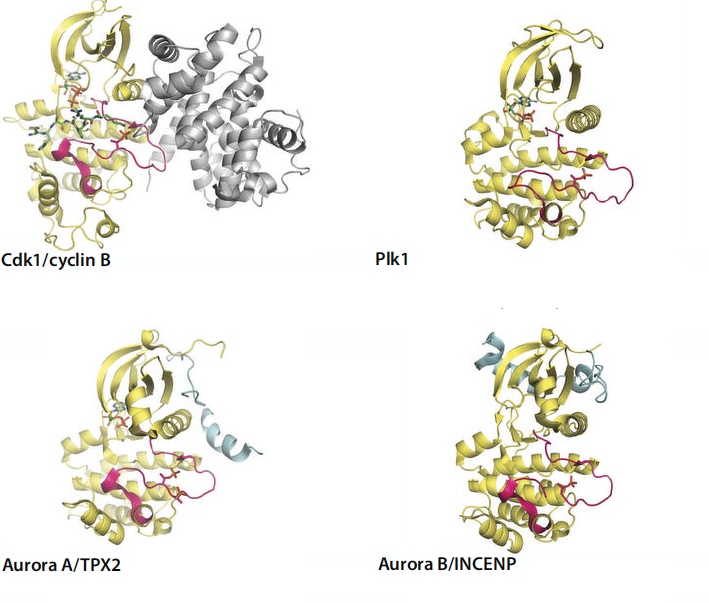
\includegraphics[height=.8\textheight]{images/Phospho/kinases_3.png}}\\}%
%   \only<3|handout:1>{\optional{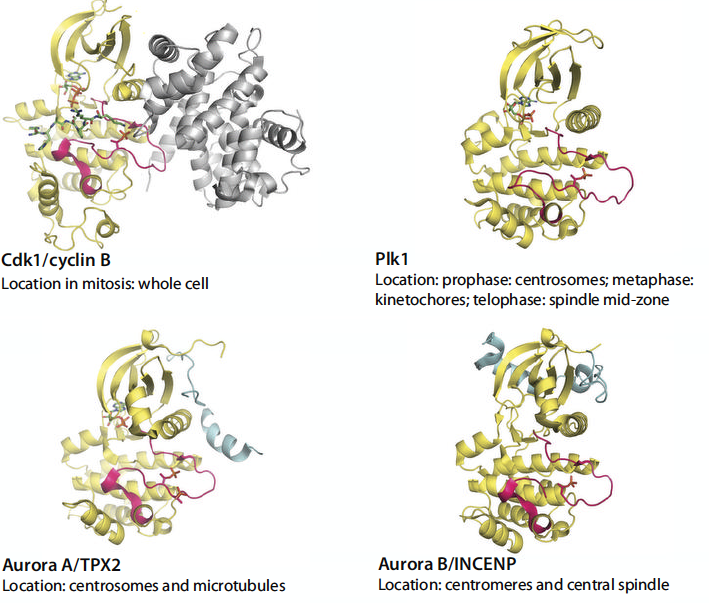
\includegraphics[height=.8\textheight]{images/Phospho/kinases_2.png}}\\}%
\end{center}
\Paper{Spatial exclusivity combined with positive and negative selection of phosphorylation motifs is the basis for context-dependent mitotic signaling}{Alexander\,et\,al.}{Sci.\,Sig\,2011}
\end{frame}

\begin{frame}[t]\frametitle{\insertsection}%
\note{~}
  \only<1-3>{%
    \begin{tabu} to \linewidth {r|ccccccc}%
      Kinase &-3&-2&-1&0&1&2&3\\\hline%
      Cdk1&.&.&.&p[ST]&P&.&[KR]\\
      Plk1&.&[DEN]&.&p[ST]&[ILMVFWY]&.&.\\
      Nek2&[FML]&[!P]&[!P]&p[ST]&[ILMV]&.&.\\
      AuroraA&R&[KR]&.&p[ST]&[!P]&.&.\\
      AuroraB&.&R&[KR]&p[ST]&[!P]&.&.\\
       \end{tabu}
    }
       \only<2|handout:0>{\vspace{0.4cm}\optional{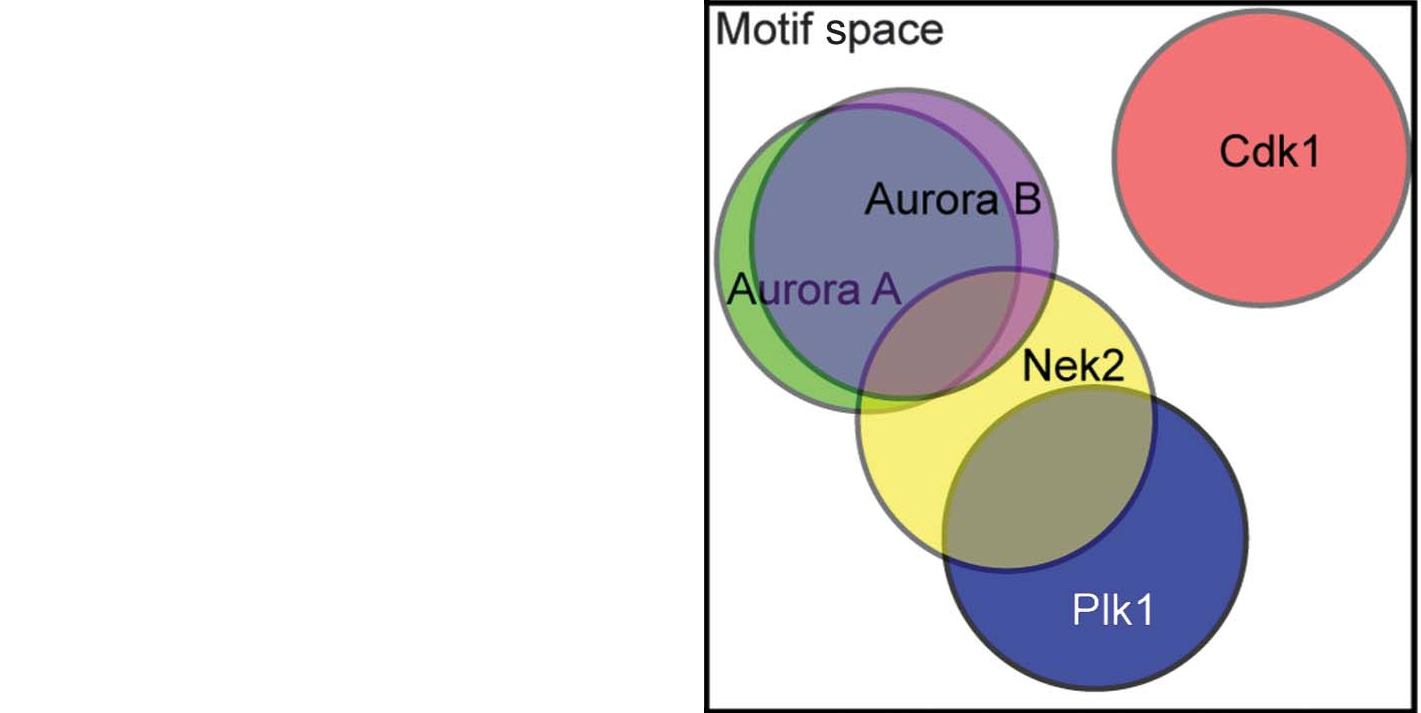
\includegraphics[width=.89\textwidth]{images/Phospho/kinase_space1.png}}}%
       \only<3|handout:1>{\vspace{0.4cm}\optional{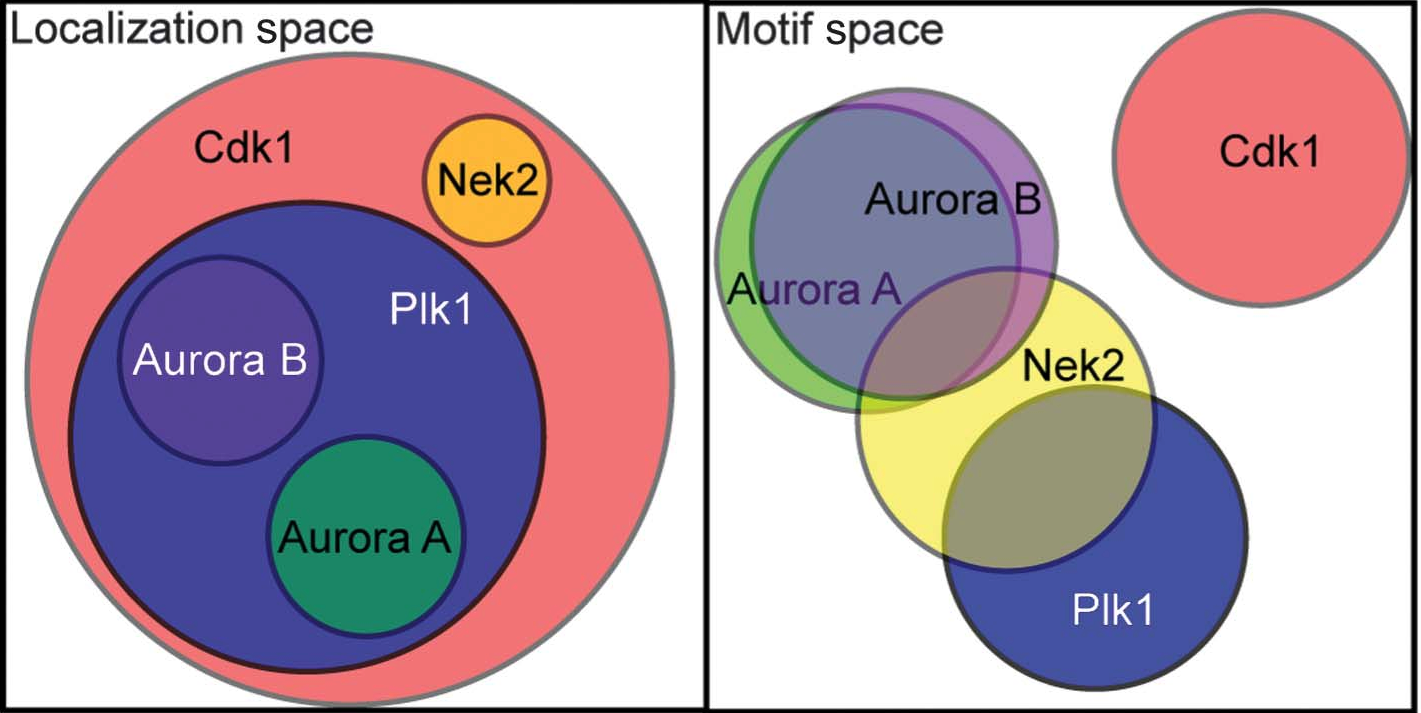
\includegraphics[width=.89\textwidth]{images/Phospho/kinase_space2.png}}}\\
         \only<4|handout:0>{%
           \begin{columns}
           \column{.4\textwidth}
           \optional{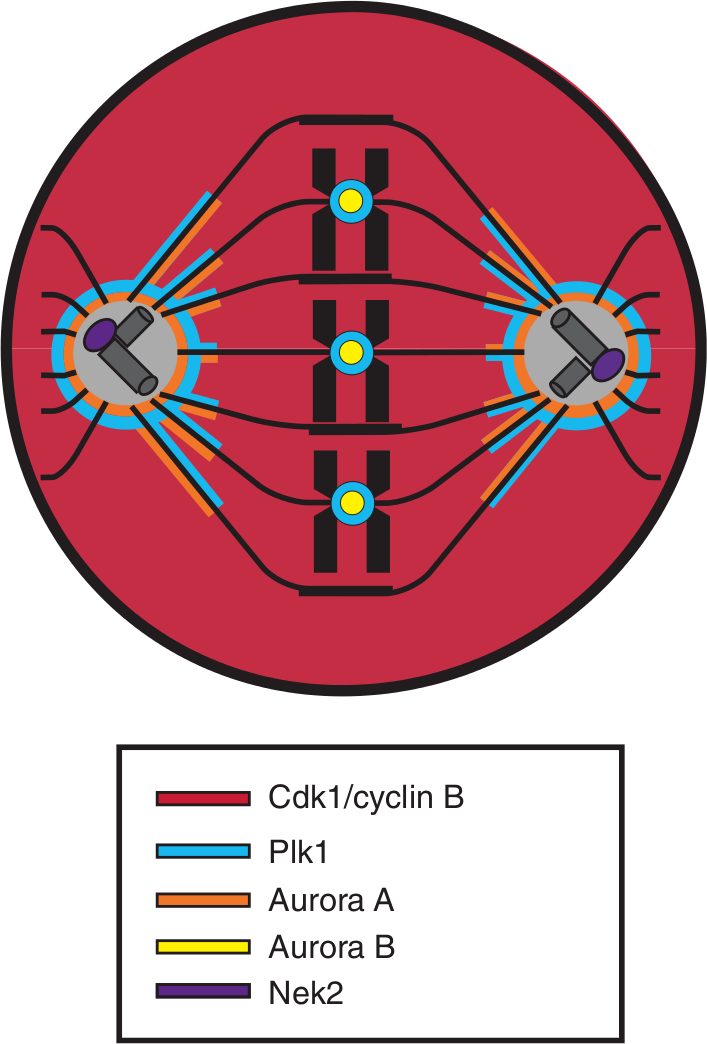
\includegraphics[height=.7\textheight]{images/Phospho/kinase_location.png}}
           \column{.6\textwidth}
           Kinase localization in Metaphase:\\
            \begin{tabular}{rl}
             \textbf{\color{red}Cdk1}& whole cell\\ 
             \textbf{\color{Cyan}Plk1}& kinetochores\\
             \textbf{\color{orange}Aurora A}& centrosomes \& microtubules\\
             \textbf{\color{Goldenrod}Aurora B}& centromeres \& spindle\\
             \textbf{\color{Fuchsia}Nek2}& centrosomes\\
             \end{tabular}
             \end{columns}
         }\\
\Paper{Spatial exclusivity combined with positive and negative selection of phosphorylation motifs is the basis for context-dependent mitotic signaling}{Alexander\,et\,al.}{Sci.\,Sig\,2011}
\end{frame}

\section{Phospho.ELM}
\begin{frame}[t]\frametitle{\insertsection}%
    \phosphoelmlogo
        %        \optional{
\includegraphics[width=.5\textwidth]{images/Phospho/Phospho_ELM_logo.png}}\\%
        \note{Phospho.ELM is mainly manually curated!}
        \only<1>{\begin{block}{Phospho.ELM}
            Database of experimentally verified phosphorylation sites in eukaryotic proteins. \\
            Current release contains 8,718 protein entries covering more than 42,500 instances.
            (Instances are fully linked to literature references.)
        \end{block}}
        \begin{center}
            \only<2|handout:1>{\optional{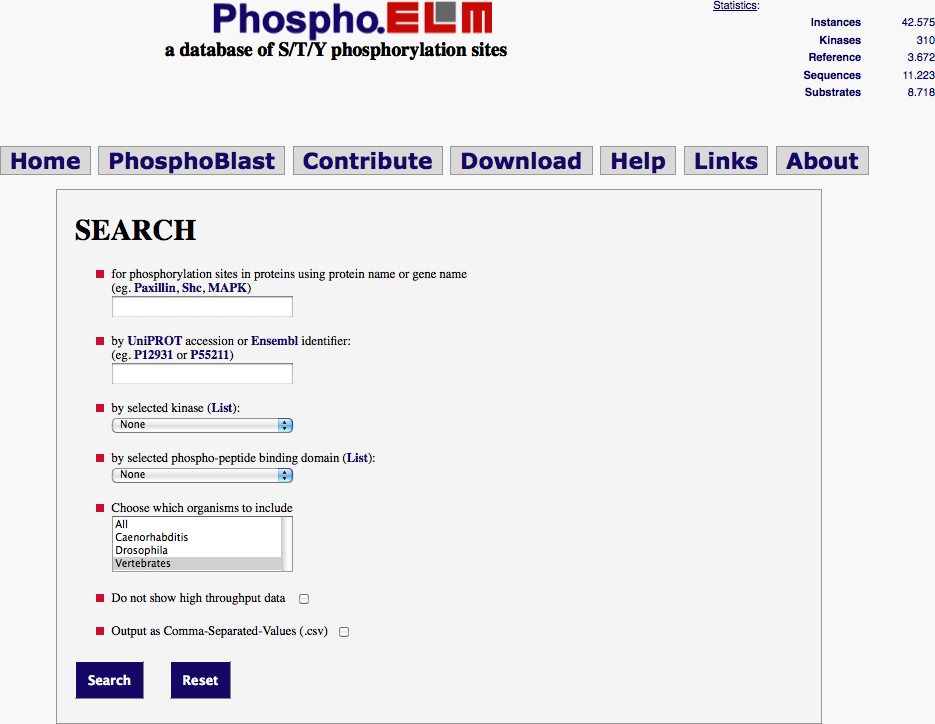
\includegraphics[width=.9\textwidth]{images/Phospho/Phospho_startpage_elm.png}}}%
        \end{center}
\end{frame}

\begin{frame}[t]\frametitle{\insertsection}%
    \phosphoelmlogo
        \note{~}
        \begin{center}
            \only<1|handout:0>{\optional{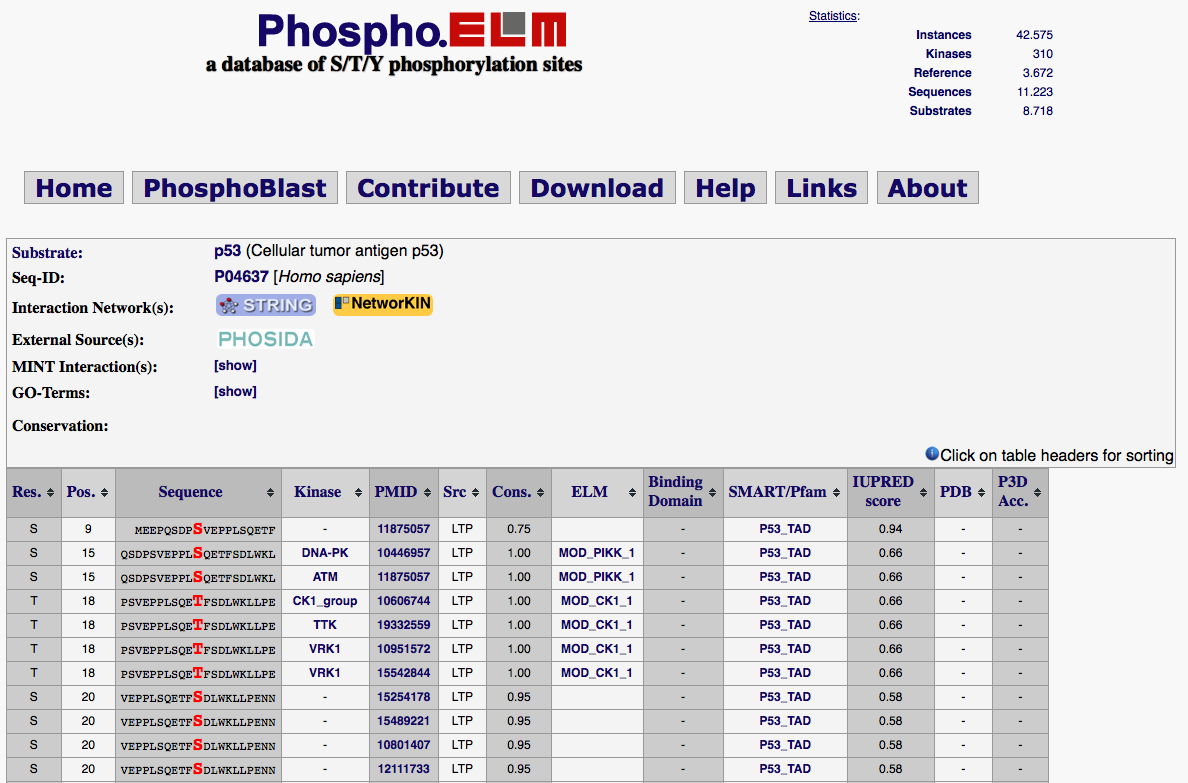
\includegraphics[width=.99\textwidth]{images/Phospho/Phospho_p53_silver.png}}}%
            \only<2|handout:1>{\optional{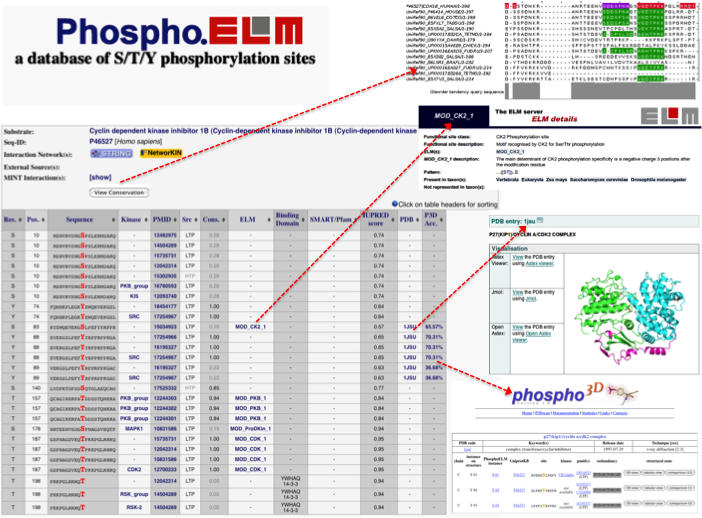
\includegraphics[width=.95\textwidth]{images/Phospho/pELM_2011_figure_1.png}}}%
        \end{center}
\end{frame}

\subsection{Link Out To Other Databases}
\begin{frame}[t]\frametitle{\insertsubsection}
    \phosphoelmlogo
    \note{~}
        \begin{columns}
            \column{.35\textwidth}
            \begin{exampleblock}{Links to:}
                \begin{itemize}
                    \item STRING
                    \item NetworKin
                    \item Phosida
                    \item Phospho3D
                \end{itemize}
            \end{exampleblock}
            \begin{exampleblock}{Display:}
                \begin{itemize}
                    \item MINT interactions
                    \item GO-Terms
                \end{itemize}
            \end{exampleblock}
            \column{.6\textwidth}
        \optional{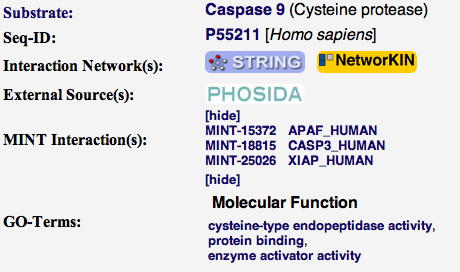
\includegraphics[width=\textwidth]{images/Phospho/Phospho_header.png}}\\ 
        \end{columns}
\end{frame}

\subsection{View Conservation in Jalview}
%\begin{frame}[t]\frametitle{
\includegraphics[width=.4\textwidth]{images/Phospho/Phospho_ELM_logo.png}~\insertsubsection}
\begin{frame}[t]\frametitle{\insertsubsection}
    \phosphoelmlogo
    \note{~}
    \begin{center}
        \only<1->{\begin{block}{}
        Precalculated conservation scores for the phosphorylation sites are presented using \structure{Jalview}
        \end{block}}
        \only<1>{\optional{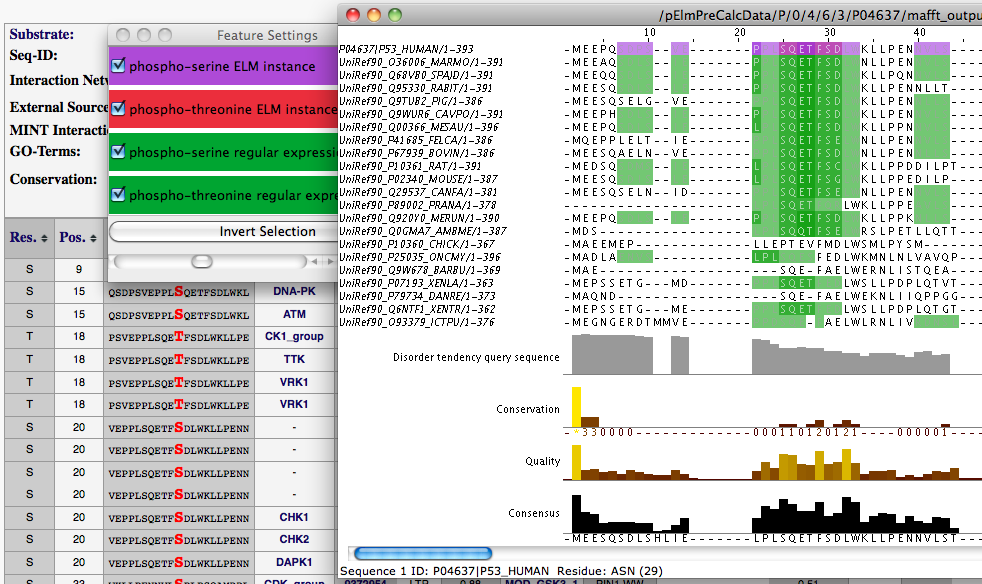
\includegraphics[width=.9\textwidth]{images/Phospho/Phospho_p53_jalview2.png}}}
    \end{center}
\end{frame}

\subsection{PhosphoSitePlus}
\begin{frame}[t]\frametitle{\insertsubsection}
    \phosphositepluslogo
    \note{~}
    \vspace*{-0.3cm}
    \begin{center}
        \only<1|handout:1>{\optional{
\includegraphics[height=.95\textheight]{images/Phospho/phosphositeplus_startpage_p53.png}}}%
        \only<2|handout:0>{\optional{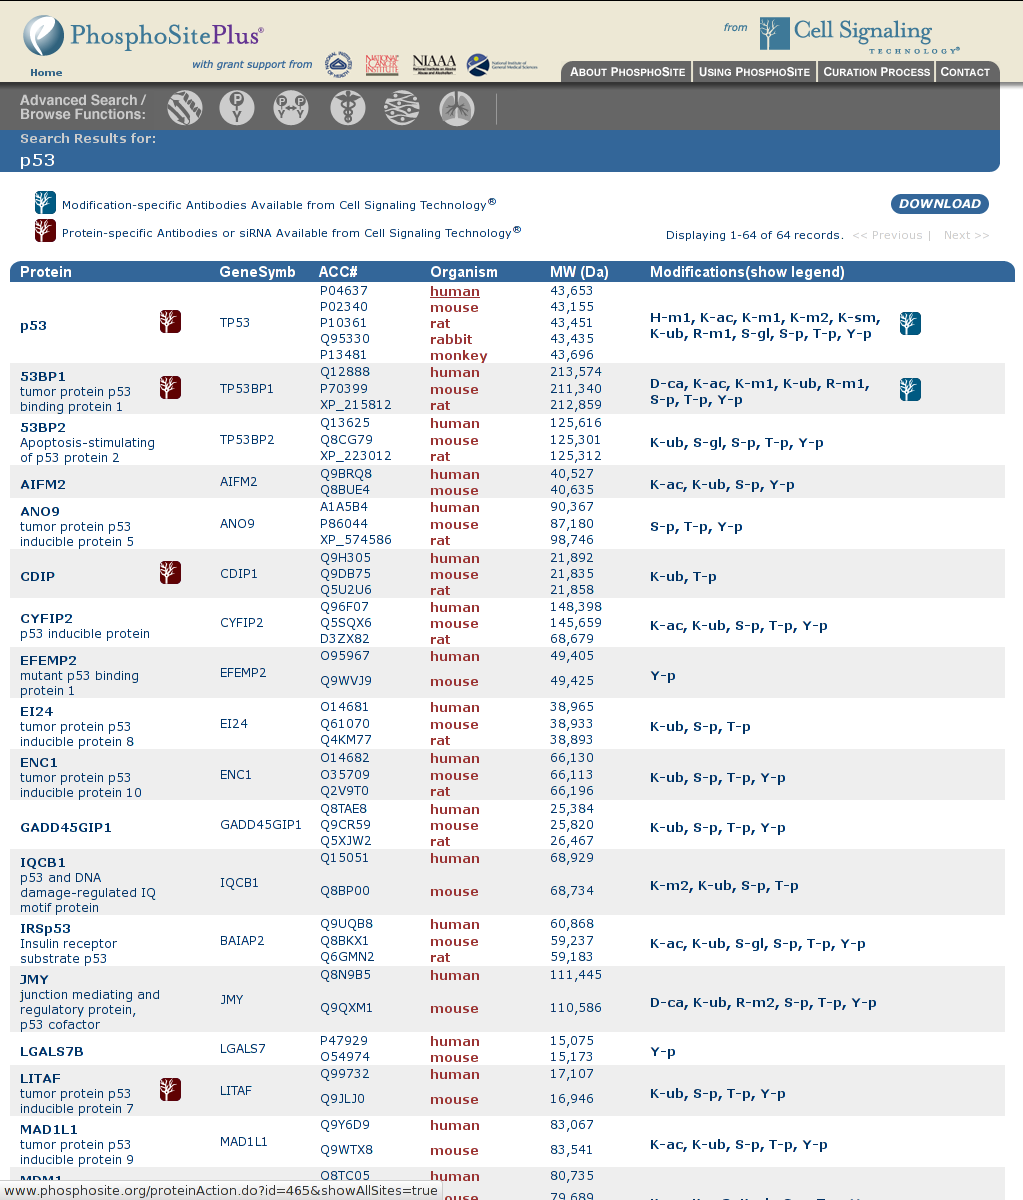
\includegraphics[height=.95\textheight]{images/Phospho/phosphositeplus_p53_list.png}}}%
        \only<3|handout:0>{\optional{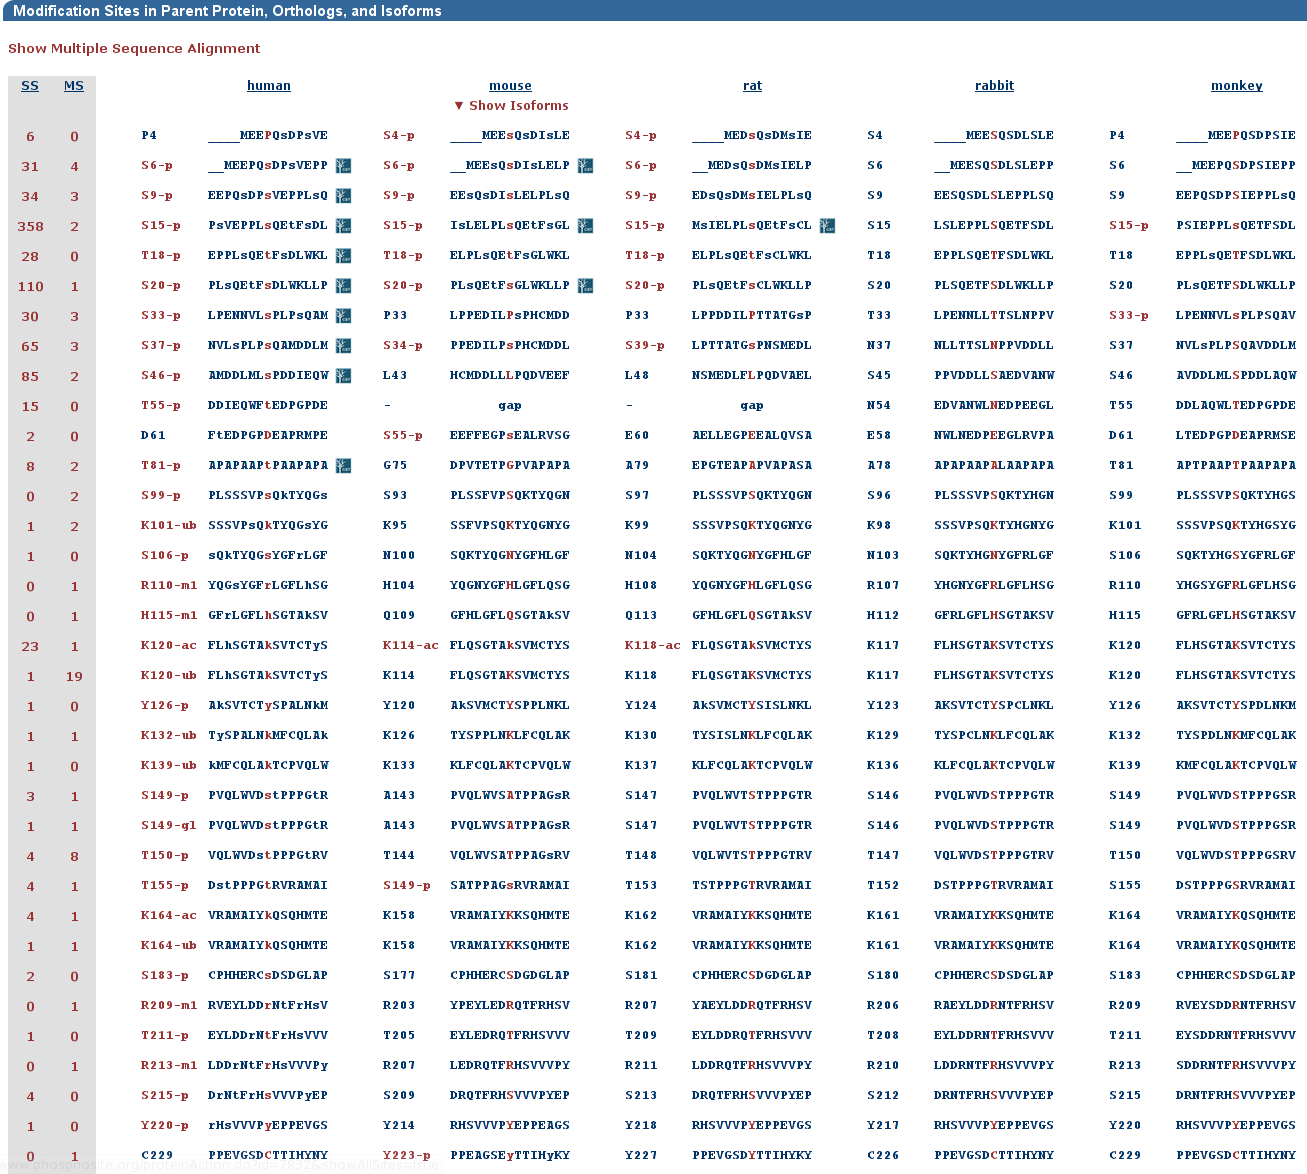
\includegraphics[height=.95\textheight]{images/Phospho/phosphositeplus_p53_detail2.png}}}%
        \only<4|handout:0>{\optional{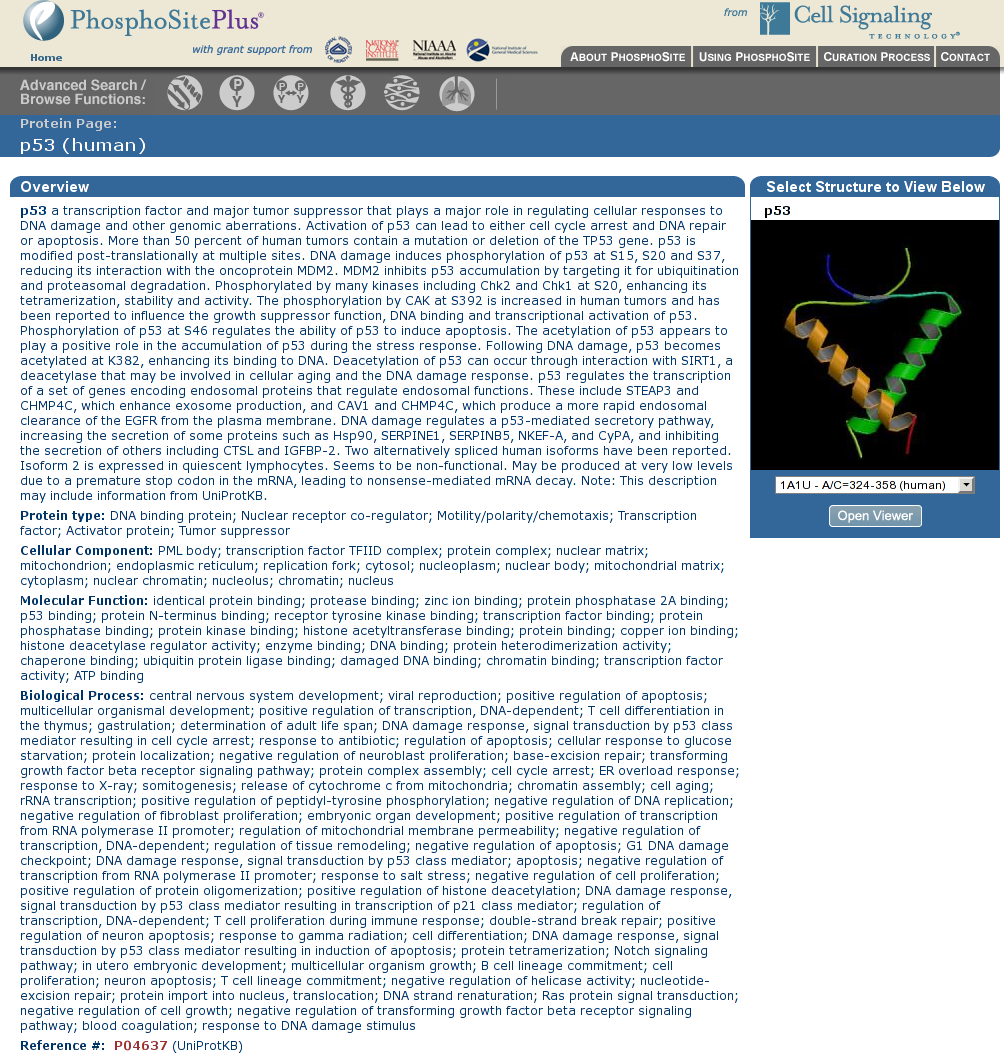
\includegraphics[height=.95\textheight]{images/Phospho/phosphositeplus_p53_detail3.png}}}%
    \end{center}
\end{frame}

\section{Questions?}
\begin{frame}<presentation:1|handout:0>[t]\frametitle{\insertsection}
    \note{~}
    \begin{center}
%      \vspace*{-1cm}
%        \optional{
\includegraphics[height=.8\textheight]{images/question_kitten.jpg}}
        \optional{
\includegraphics[height=.8\textheight]{images/curiosity-questions-answer-questions-answers-demotivational-poster-12876368551.jpg}}
    \end{center}
\end{frame}

\section{ELM}%
\subsection{The ELM server}%
\begin{frame}[t]\frametitle{\insertsubsection{}}%
    \elmlogo
    \note{By detecting \structure{functional} motifs in a protein sequence, we can put that protein into context.}
    \note{Current status of ELM. This is how ELM looks like for the user?}%
    \note{my Job: Improving the user interface and implementing new methods}%
        \visible<1->{\vspace{-2mm}
            \optional{
\includegraphics[width=.8\textwidth]{images/elm/elm_title_trans.png}}\\\vspace{-8mm}%
        \hogsboxtop{The \includegraphics[width=1cm]{elm_logo_transparent.png}~resource}{is a collection of more than 240 thoroughly annotated motif
        classes with over 2700 annotated instances. \\
        It is also a prediction tool to detect these motifs in protein sequences employing different filters to distinguish between \structure{functional}
        and \structure{non-functional} motif instances.}%
    }\medskip
    \begin{center}\vspace{-2mm}
        \only<2|handout:1>{\optional{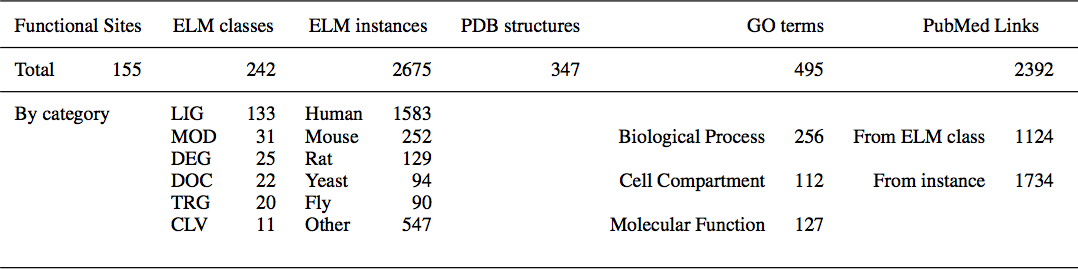
\includegraphics[width=.95\textwidth]{images/elm/table_elm_trans.png}}}%
    \end{center}
    \Paper{The eukaryotic linear motif resource ELM: 10 years and counting}{Dinkel, van~Roey, Michael, Davey, Weatheritt, Born, Speck, Kr"uger, Grebnev, Kuba\'{n}, Strumillo, Uyar, Budd, Altenberg, Seiler, Chemes, Glavina, S\'{a}nchez, Diella \& Gibson}{Nucleic~Acids~Res.~2014}
\end{frame}

% \begin{frame}\frametitle{ELM History}
%     \elmlogo
%     \note{
%     creation\_date \& modifying\_time (last time an entry has been updated.\\
%     recent modifications: mainly Kim updating the database, adding information, fixing errors...\\
%     }
%     \begin{center}
%         \vspace{-2mm}\optional{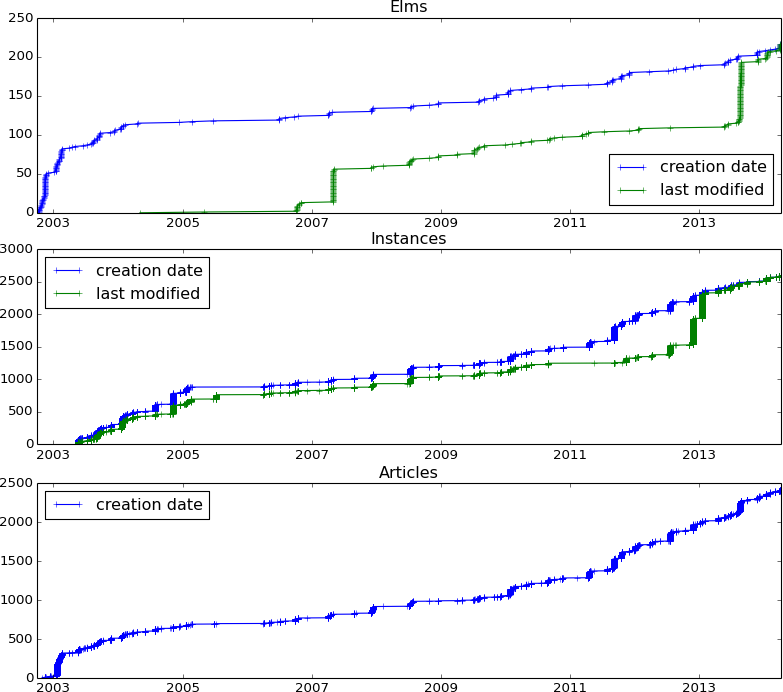
\includegraphics[height=.9\textheight]{images/plot_elm_history.png}}
%     \end{center}
% \end{frame}

\begin{frame}[t]\frametitle{The ELM Database}
    \elmlogo
    \note{ ELM class describes a linear motif class. Information curated from literature.\\
    Instances are experimentally verified instances of ELM classes. Annotated with experimental methods, References etc.\\
    Recently added interaction data to ELM database\\
    }
    \begin{columns}[T]
        \begin{column}{.49\textwidth}
            \begin{block}{ELM Class}
                Condensed information about a motif. Regular Expressions used to annotate the motif (eg. ''{\verb x[KR]xLx\{0,1\}[FYLIVMP]}" for Cyclin motif)
            \end{block}
            \only<2>{\optional{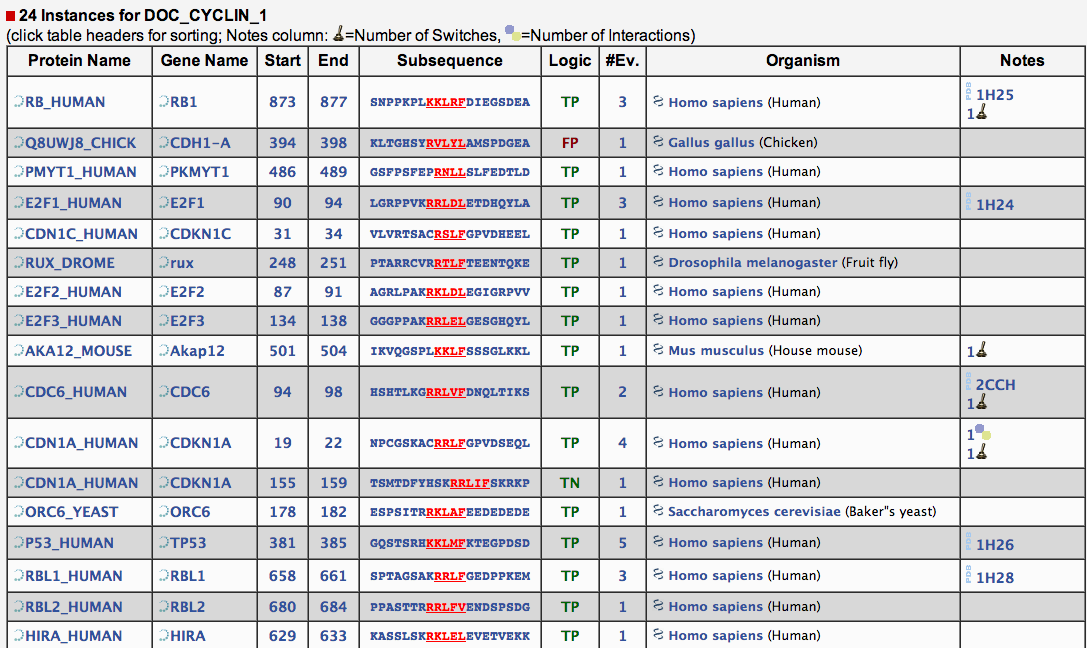
\includegraphics[width=\textwidth]{images/Cyclin_Instances.png}}}
            \only<3->{\optional{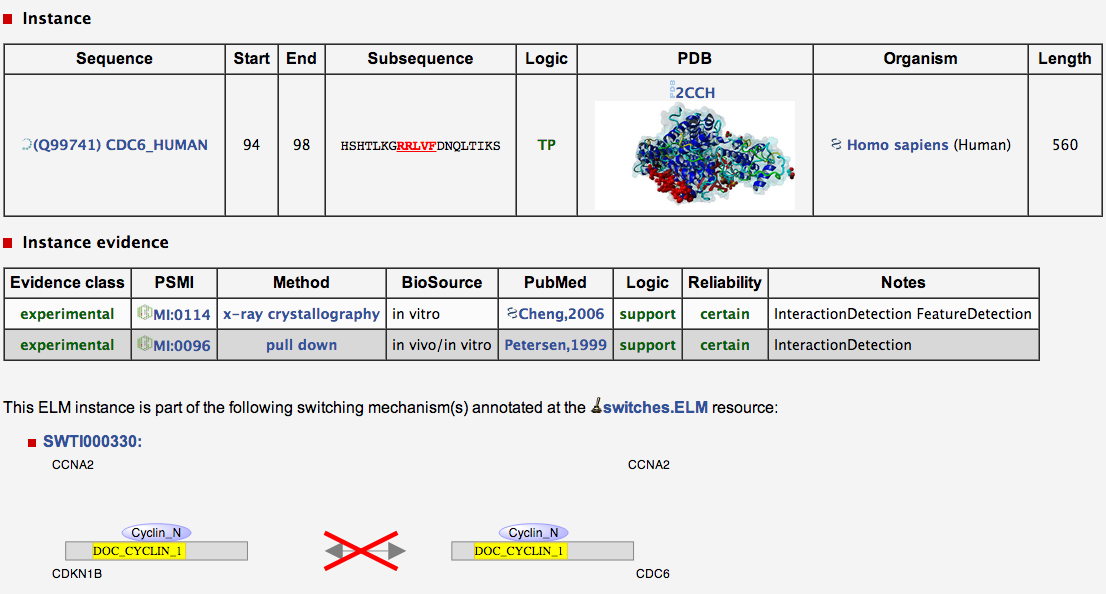
\includegraphics[width=\textwidth]{images/Cyclin_Instance_Detail.png}}}
        \end{column}
        \begin{column}{.49\textwidth}
            \optional{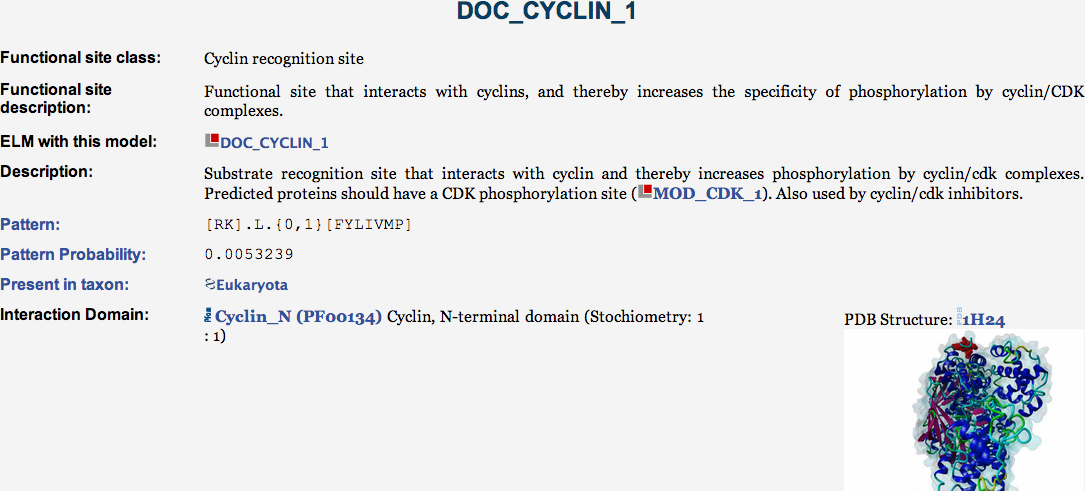
\includegraphics[width=\textwidth]{images/Cyclin_Class.png}}
            \visible<2->{
            \begin{exampleblock}{ELM Instance}
                An experimentally verified instance of an ELM class in a particular sequence.
                \visible<3->{
                \begin{itemize}
                    \itemsep0pt\parskip0pt\parsep0pt
                    \item<4-> Experimental Evidences
                    \item<5-> Methods
                    \item<6-> References
                    \item<7-> Interactions
                \end{itemize}
            }
            \end{exampleblock}
            }
        \end{column}
    \end{columns}
    \only<7->{\Paper{iELM -- a web server to explore short linear motif-mediated interactions.}{Weatheritt, Jehl, \underline{\textbf{Dinkel}} \& Gibson }{Nucleic~Acids~Res.~2012}}%
\end{frame}

\subsection{ELM database}
\begin{frame}[t]\frametitle{\insertsubsection{}}%
    \elmlogo
    \begin{center}\vskip-1.1em%
        \only<1|handout:0>{\optional{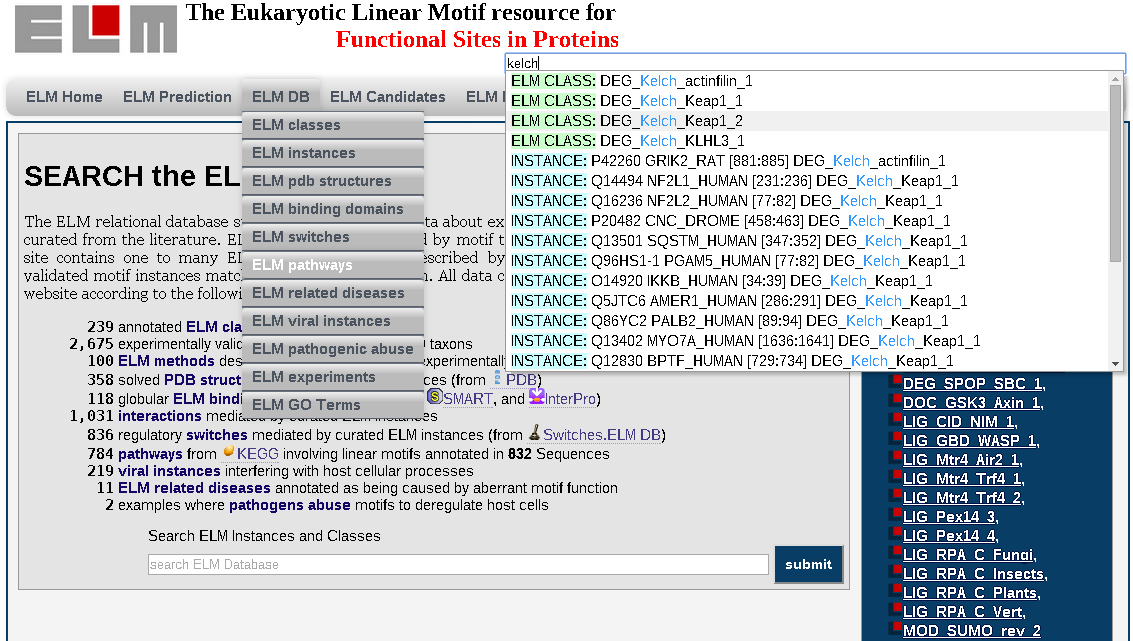
\includegraphics[width=.9\textwidth]{images/elm/elm_screenshot_autocomplete.png}}}%
        \only<2|handout:1>{\optional{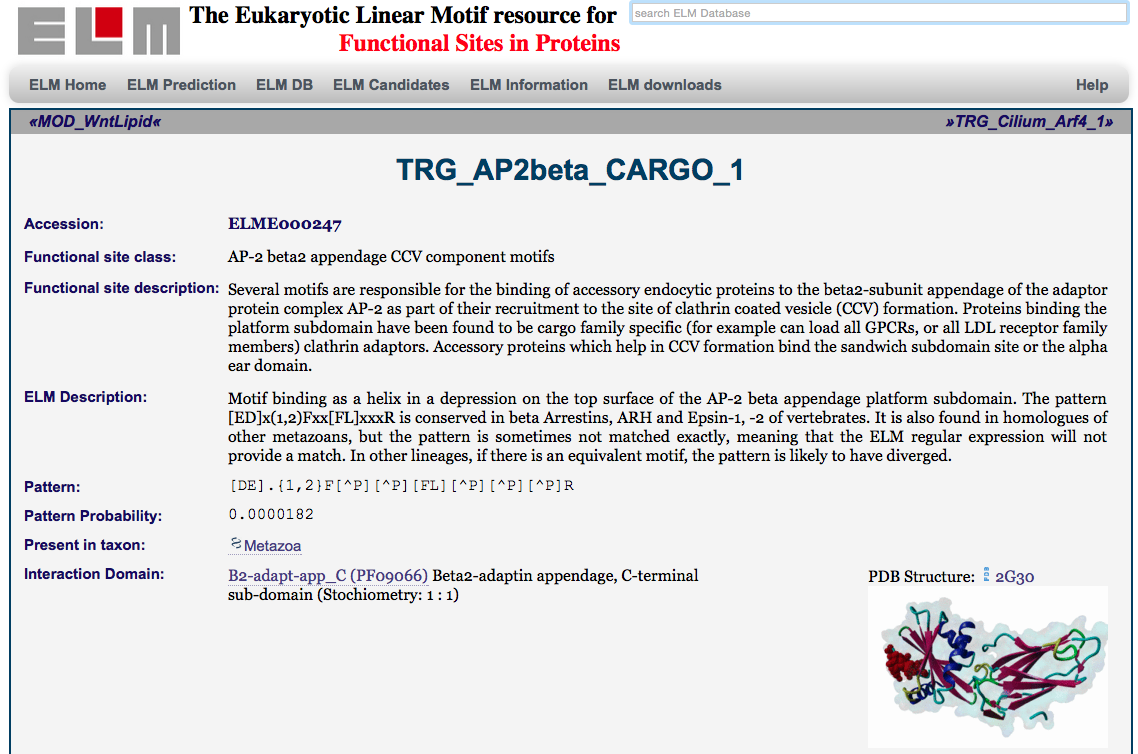
\includegraphics[width=.9\textwidth]{images/elm/Figure3.png}}}%
        \only<3|handout:0>{\optional{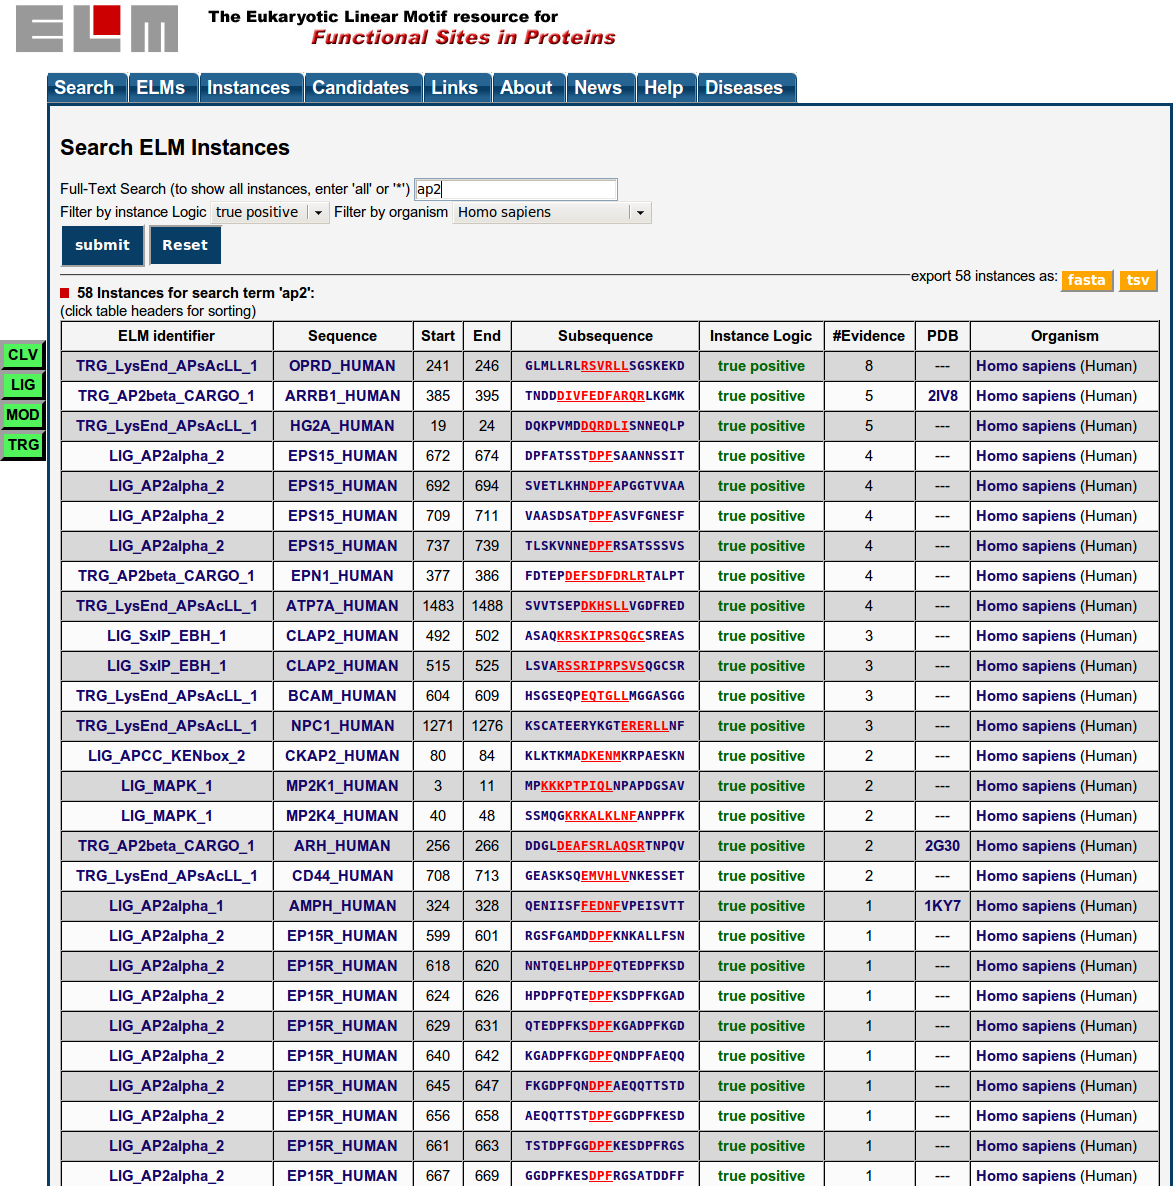
\includegraphics[width=.9\textwidth]{images/elm/Figure4.png}}}%
    \end{center}%
\end{frame}

\subsection{ELM database:Diseases}
\begin{frame}[t]\frametitle{\insertsubsection{}}%
    \elmlogo
    \begin{center}\vskip-1.1em%
        \optional{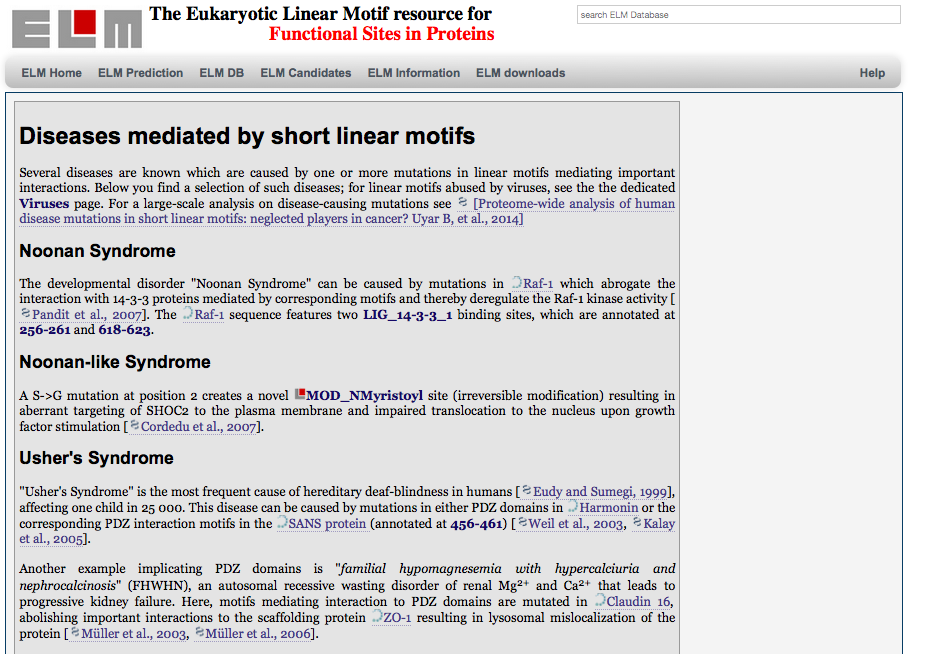
\includegraphics[width=.9\textwidth]{images/elm/ELM_diseases_page.png}}%
    \end{center}%
\end{frame}

% \subsection{ELM database:Viruses}
% \begin{frame}[t]\frametitle{\insertsubsection{}}%
%     \elmlogo
%     \begin{center}\vskip-1.1em%
%         \optional{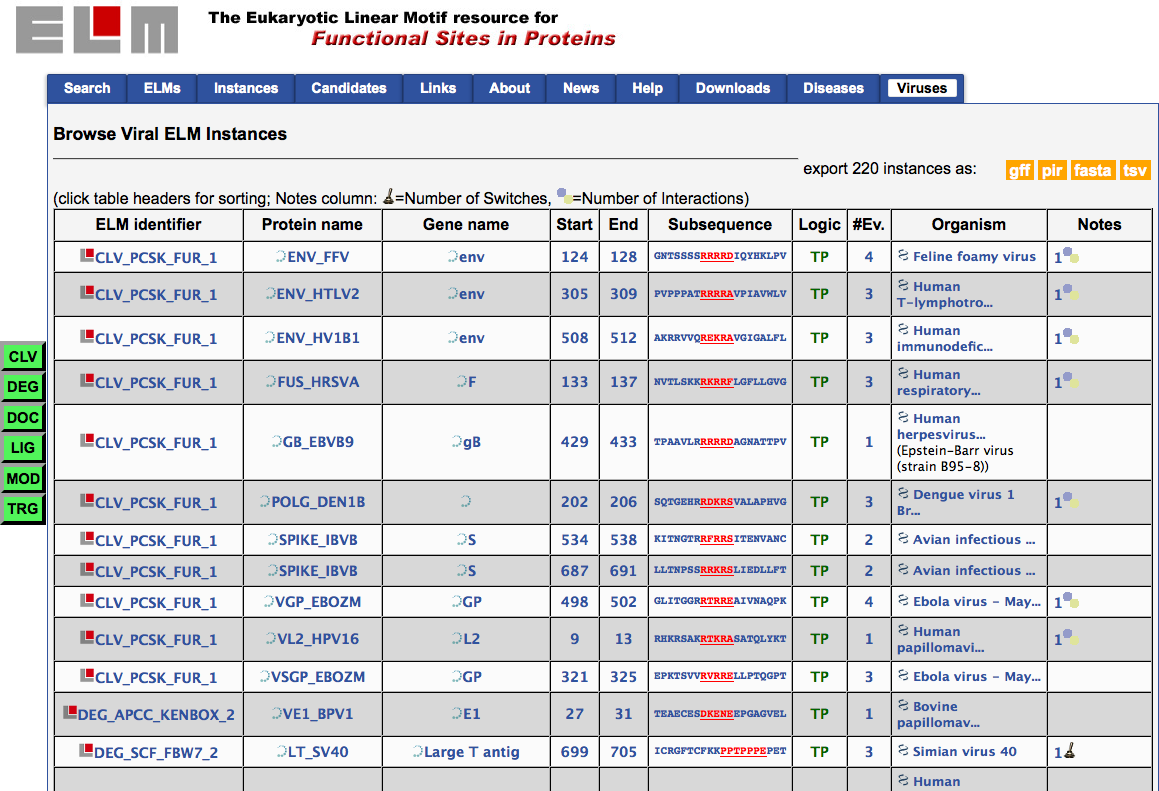
\includegraphics[width=.9\textwidth]{images/elm/ELM_virus_page.png}}%
%     \end{center}%
% \end{frame}


\subsection{ELM database:Pathways}
\begin{frame}[t]\frametitle{\insertsubsection{}}%
    \elmlogo
    \begin{center}\vskip-1.1em%
        \optional{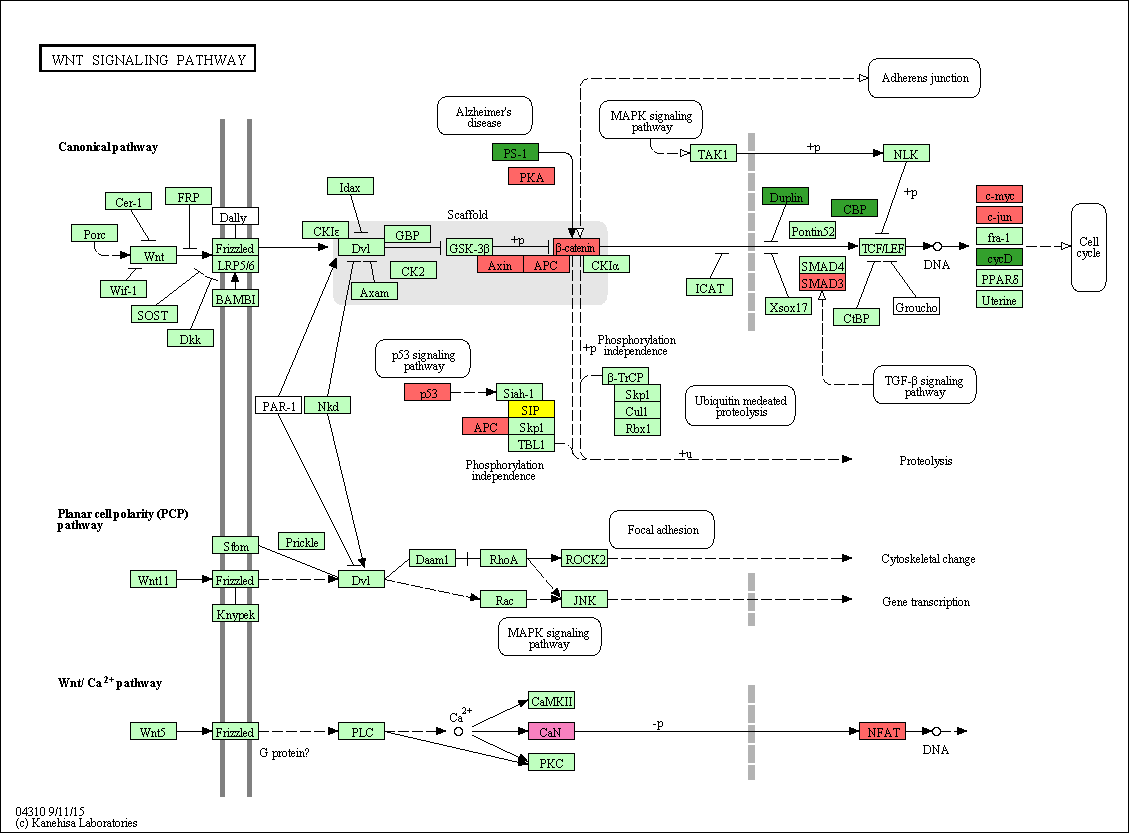
\includegraphics[width=.95\textwidth]{images/elm/kegg_wnt_pathway.png}}%
    \end{center}%
\end{frame}

\subsection{ELM prediction tool}
\begin{frame}[t]\frametitle{\insertsubsection{}}%
    \elmlogo
    \begin{center}\vskip-1.1em%
        \only<1|handout:1>{\optional{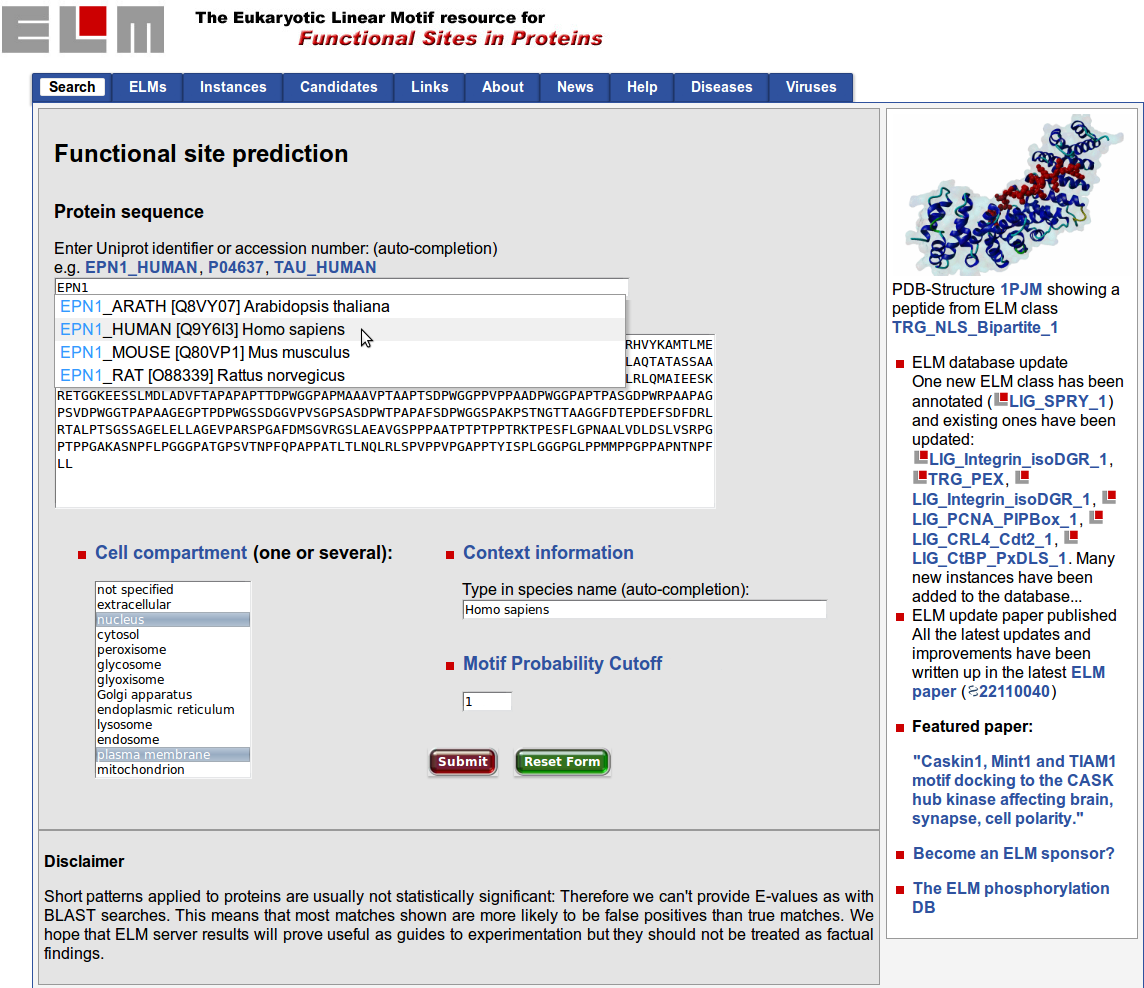
\includegraphics[width=.9\textwidth]{images/elm/ELM_startpage.png}}}%
    \end{center}%
\end{frame}
\begin{frame}[t]\frametitle{\insertsubsection{}}%
    \elmlogo
    \begin{center}\vskip-1.1em%
        \only<1|handout:1>{\optional{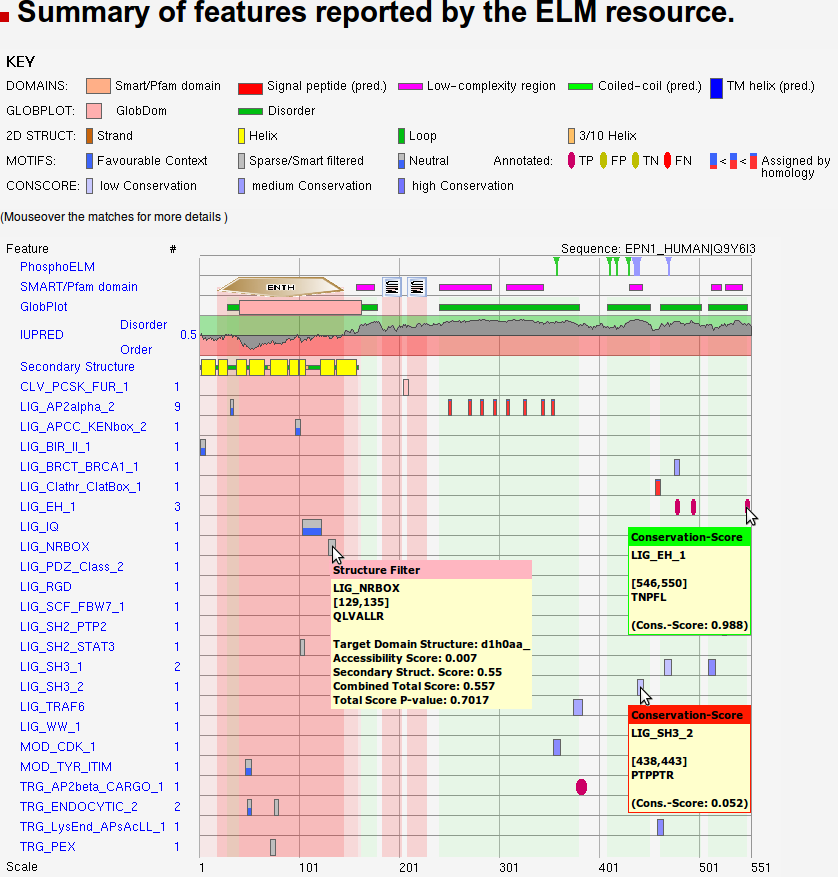
\includegraphics[width=.9\textwidth]{images/elm/Figure2.png}}}%
    \end{center}%
\end{frame}

\subsection{View Conservation in Jalview}
\begin{frame}[t]\frametitle{\insertsubsection}
    \elmlogo
    \note{~}
    \begin{center}
        \only<1>{\optional{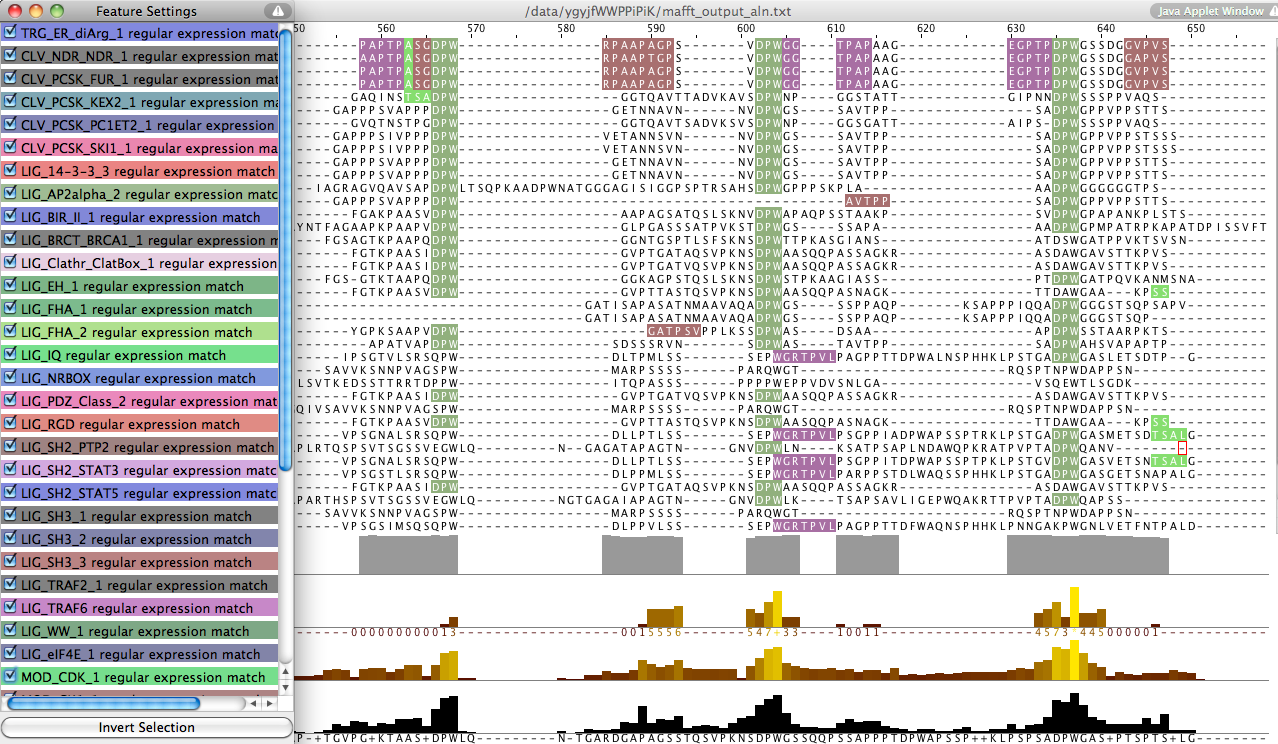
\includegraphics[width=.98\textwidth]{images/elm/Jalview.png}}}
    \end{center}
\end{frame}

\section{Questions?}
\begin{frame}<presentation:1|handout:0>[t]\frametitle{}
    \note{~}
    \begin{center}
      \vspace*{-0.5cm}\huge{Questions?}
        \optional{
\includegraphics[height=.8\textheight]{images/curiosity.jpg}}
    \end{center}
\end{frame}

\section{Linear Motifs as Molecular Switches}
\begin{frame}\frametitle{\insertsection}
    \visible<+->{\begin{exampleblock}{Short Linear Motifs}
        \begin{itemize}
            %        \item are a spatially efficient and convergently evolvable solution for encoding interaction interfaces.
            \item are compact, degenerate protein interaction interfaces (in IDRs)
            \item are ubiquitous in eukaryotic proteomes and mediate many regulatory functions:
                \begin{itemize}
                    \item directing ligand binding
                    \item providing docking sites for modifying enzymes
                    \item controlling protein stability
                    \item acting as signals to target proteins to specific subcellular locations
                \end{itemize}
%            \item Typically, only 3--4 residues of a SLiM determine the majority of the binding specificity \& affinity
        \end{itemize}
    \end{exampleblock}}
    \visible<+->{\begin{block}{Motif-mediated interactions}
        \begin{itemize}
            \item occur with low affinity, 
            \item are transient \& reversible
            \item can be easily modulated. 
        \end{itemize}
    \end{block}}
    \visible<+->{\begin{alertblock}{Motifs mediate switches}
        This makes SLiMs ideal regulatory modules and enable them to conditionally \alert{switch} between ``on'' and ``off'' states or between multiple, functionally distinct on states.
%        Motif Switching can be mediated by multiple mechanisms that often depend on
%        posttranslational modifications and the cooperative or competitive use of multiple overlapping or adjacent SLiMs. 
        %Conditional switching of motif functionality can stimulate a gain, loss, or exchange of
        %binding partners and thereby regulate the function of SLiM-containing proteins in a context-dependent manner.
    \end{alertblock}}%
    \Paper{The switches.ELM Resource: A Compendium of Conditional Regulatory Interaction Interfaces}{van~Roey, Dinkel, Weatheritt, Gibson and Davey}{Science~Signaling.~2013}
\end{frame}

\begin{frame}\frametitle{\insertsection}
    \switcheslogo
    \note{~}
    \begin{center}
%    \optional{
\includegraphics[width=.2\textwidth]{images/switches/switches_elm_logo.png}}\\
%    \framezoom<1|handout:0><1|handout:0>(-0.8cm,0cm)(2cm,3cm) 
%    \framezoom<1|handout:0><2|handout:0>(3.8cm,0.8cm)(3.7cm,2cm)
    \only<1|handout:0>{\optional{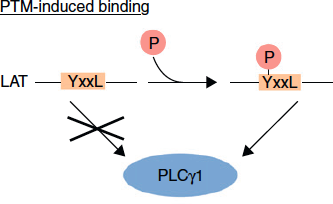
\includegraphics[width=.6\textwidth]{images/switches/switches_overview_1_1.png}}\\}
    \only<2|handout:0>{\optional{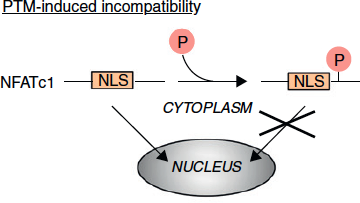
\includegraphics[width=.6\textwidth]{images/switches/switches_overview_1_2.png}}\\}
    \only<3|handout:1>{\optional{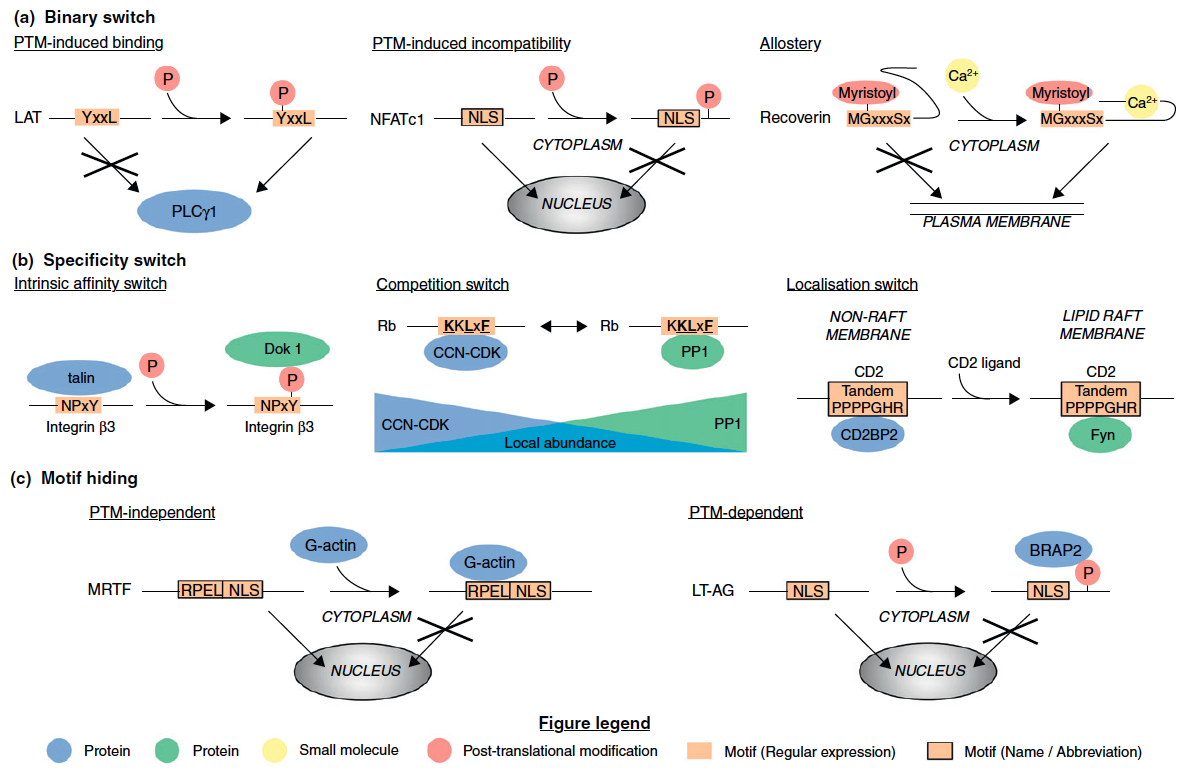
\includegraphics[width=.9\textwidth]{images/switches/switches_overview_1.png}}\\}
    \only<4|handout:0>{\optional{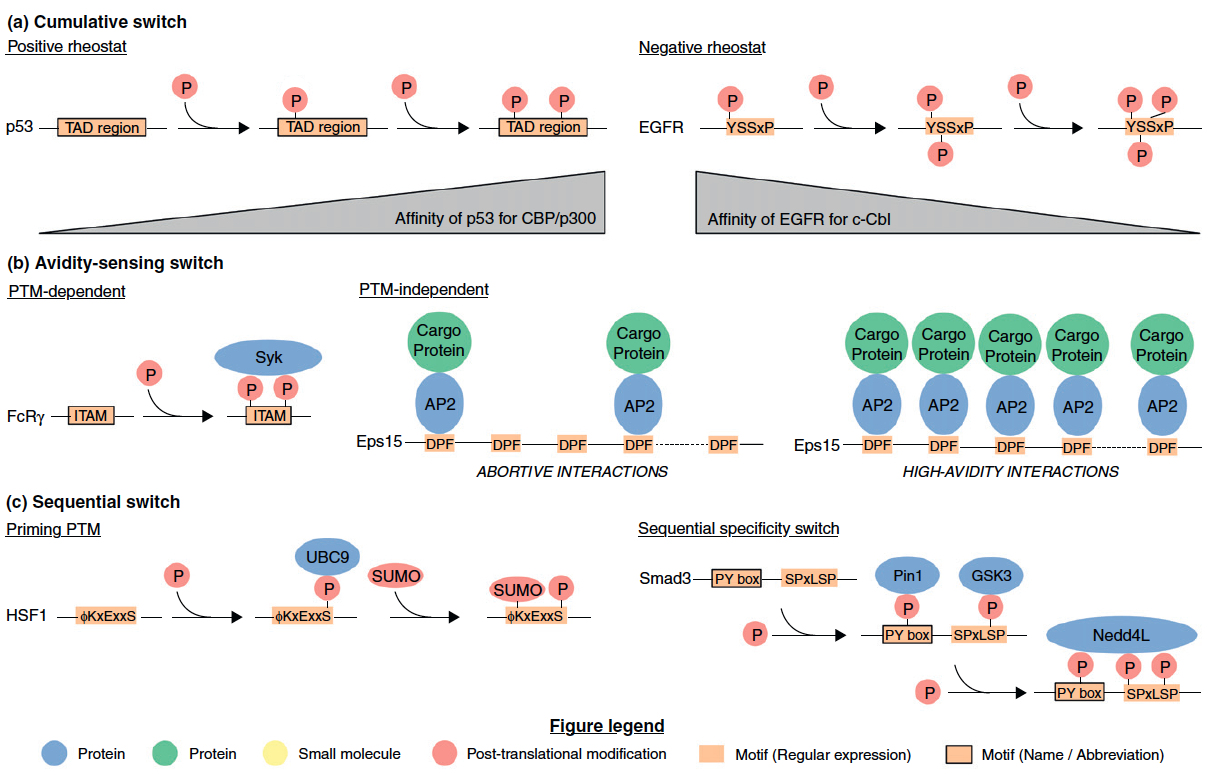
\includegraphics[width=.9\textwidth]{images/switches/switches_overview_2.png}}\\}
%    \only<5|handout:0>{\optional{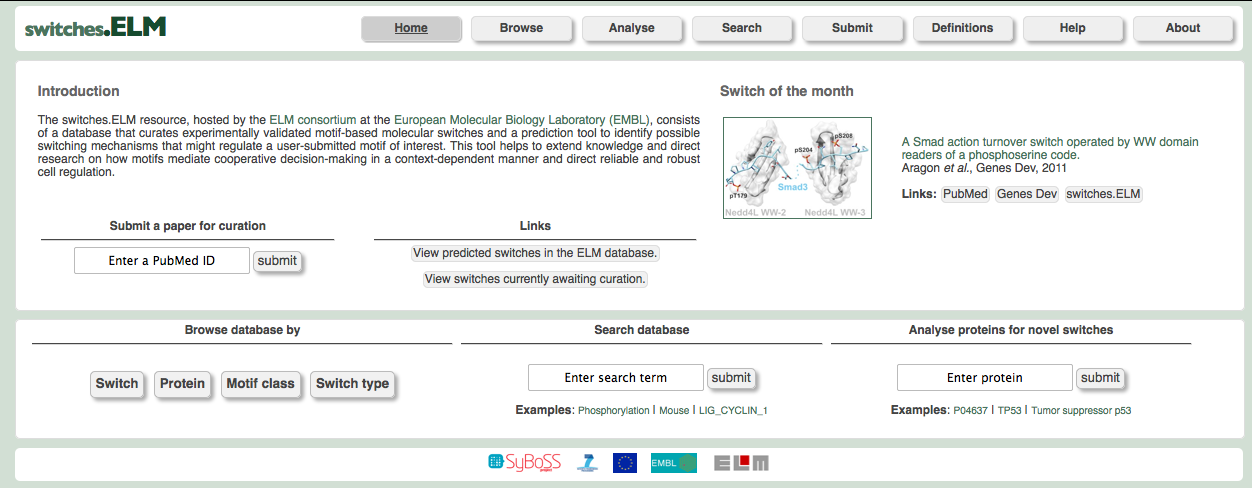
\includegraphics[width=.99\textwidth]{images/switches/switches_elm_start.png}}\\}
%    \only<6|handout:1>{\optional{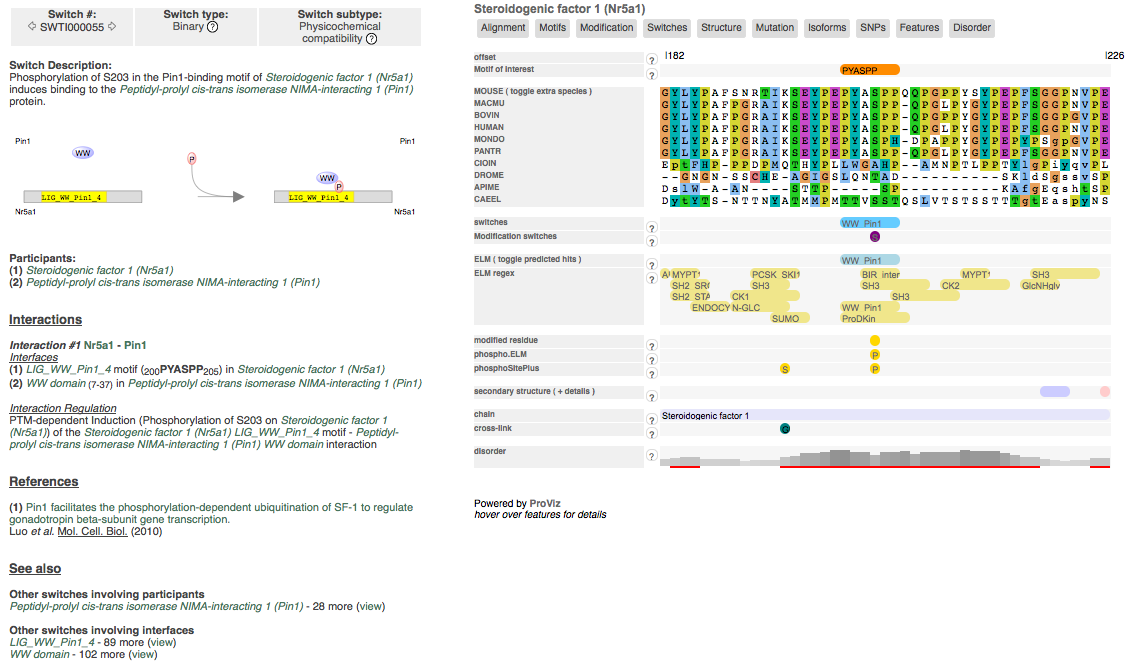
\includegraphics[width=.9\textwidth]{images/switches/switches_elm_0055.png}}\\}
    \end{center}
\end{frame}

\begin{frame}\frametitle{\insertsection}
    \switcheslogo
    \note{~}
\begin{exampleblock}{}
    The switches.ELM \alert{database} curates experimentally validated motif-based molecular switches.\\
    In addition, based on these validated instances, the switches.ELM \alert{prediction} tool was developed to identify possible switching mechanisms that might regulate a motif-containing protein of interest. 
\end{exampleblock}

    \begin{center}
    \only<1|handout:0>{\optional{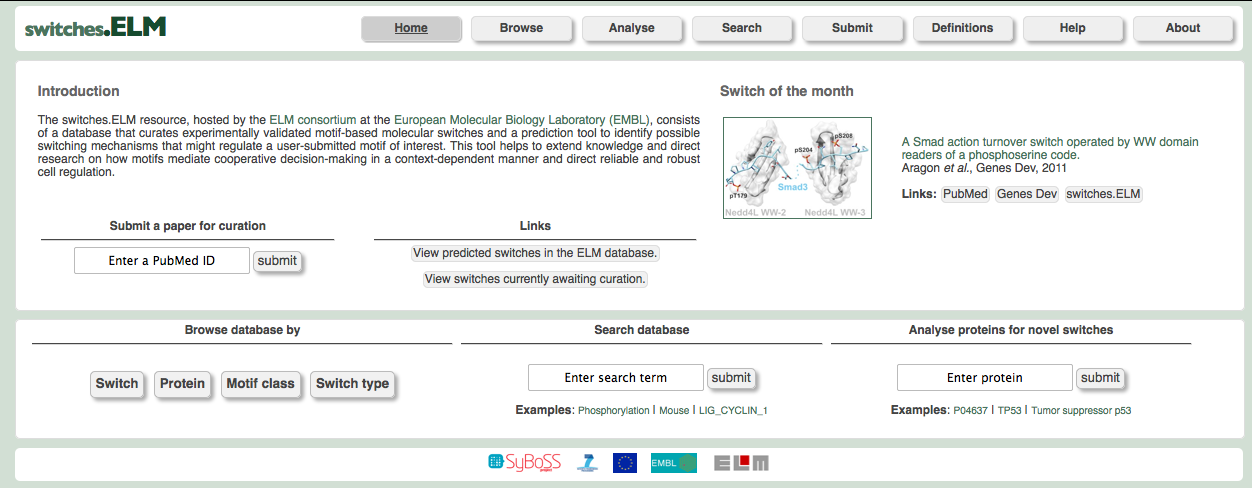
\includegraphics[width=.99\textwidth]{images/switches/switches_elm_start.png}}\\}
    \only<2|handout:1>{\optional{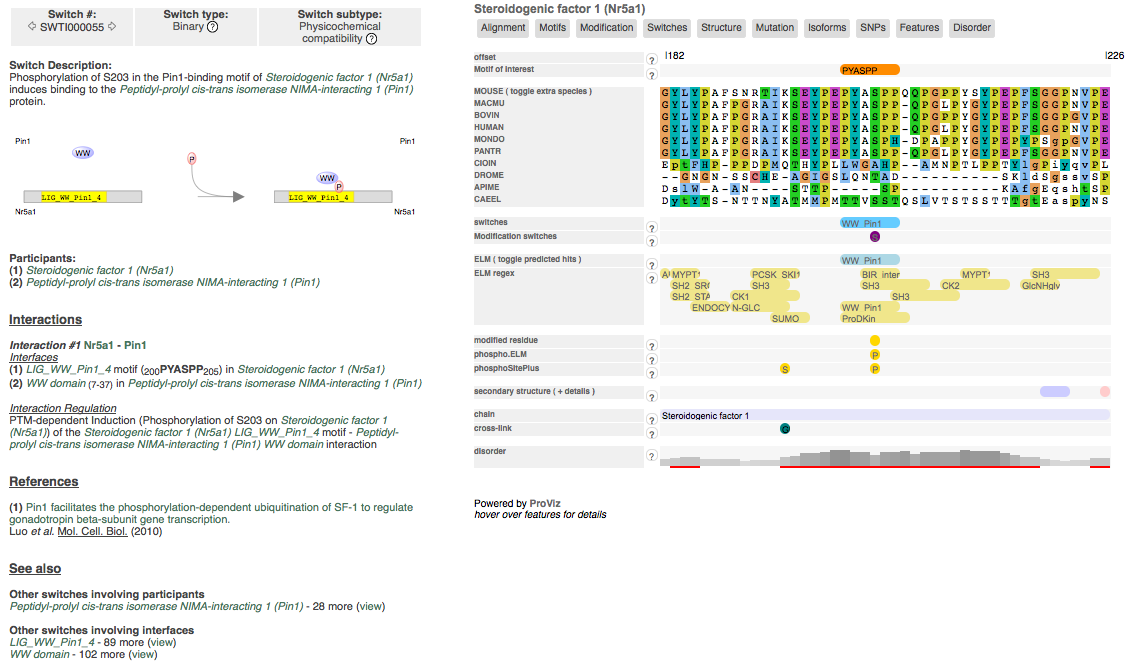
\includegraphics[width=.9\textwidth]{images/switches/switches_elm_0055.png}}\\}
    \end{center}
\end{frame}

\section{Questions?}
\begin{frame}<presentation:1|handout:0>[t]\frametitle{}
    \note{~}
    \begin{center}
      \vspace*{-0.5cm}\huge{Questions?}
        \optional{
\includegraphics[height=.8\textheight]{images/curiosity-killed-the-cat-killed-cat-demotivational-posters-1327622456.jpg}}
    \end{center}
\end{frame}


\end{document}
